\chapter{Další prostorové křivky}
Nyní si můžeme definovat nejrůznější křivky sami. Například
$$k(t)=[\cos{t}, \ln{t}\cdot\sin{t}, \ln{t}], t \in (0, +\infty),$$
\begin{figure}[H]
	\centering
	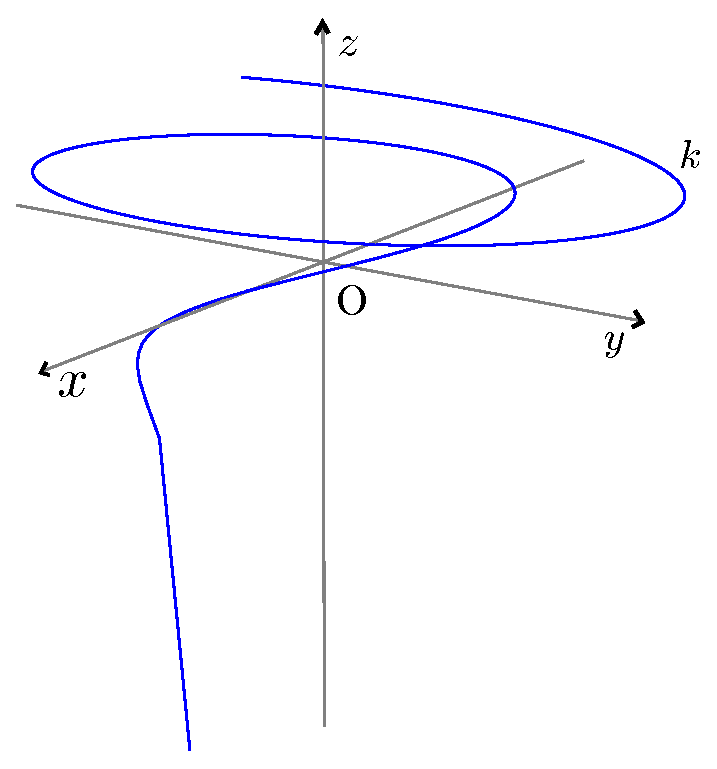
\includegraphics[width=0.275\textwidth]{prostorovekrivky-teorie1.eps}
	\caption{Křivka \textit{k} pro $t \in \left\langle\frac{1}{10}, 10\right\rangle$}
\end{figure}
$$k(t)=\left[\frac{1}{t^2+1}, \frac{t}{t^2+1}, \frac{t^2}{t^2+1}\right], t \in \mathbb{R},$$
\begin{figure}[H]
	\centering
	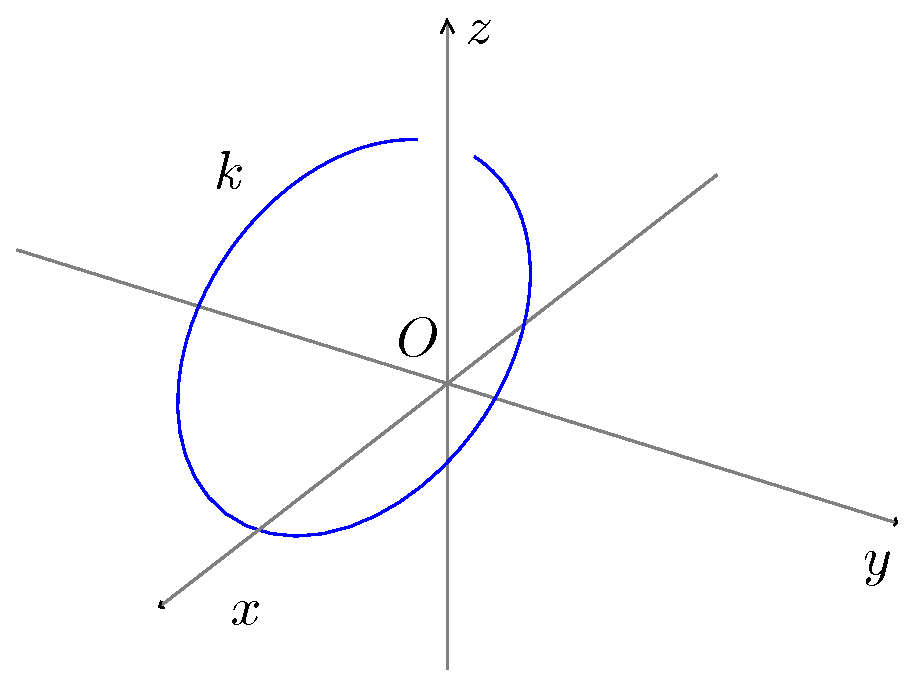
\includegraphics[width=0.28\textwidth]{prostorovekrivky-teorie2.eps}
	\caption{Křivka \textit{k} pro $t \in \langle-10,10\rangle$}
\end{figure}
(je to elipsa v rovině $x+z-1=0$), \clearpage{}
\noindent{}$$k(t)=[\sinh{t}, \cosh{t}, \sin{6t}], t \in \langle-\pi, \pi\rangle.$$
\begin{figure}[H]
	\centering
	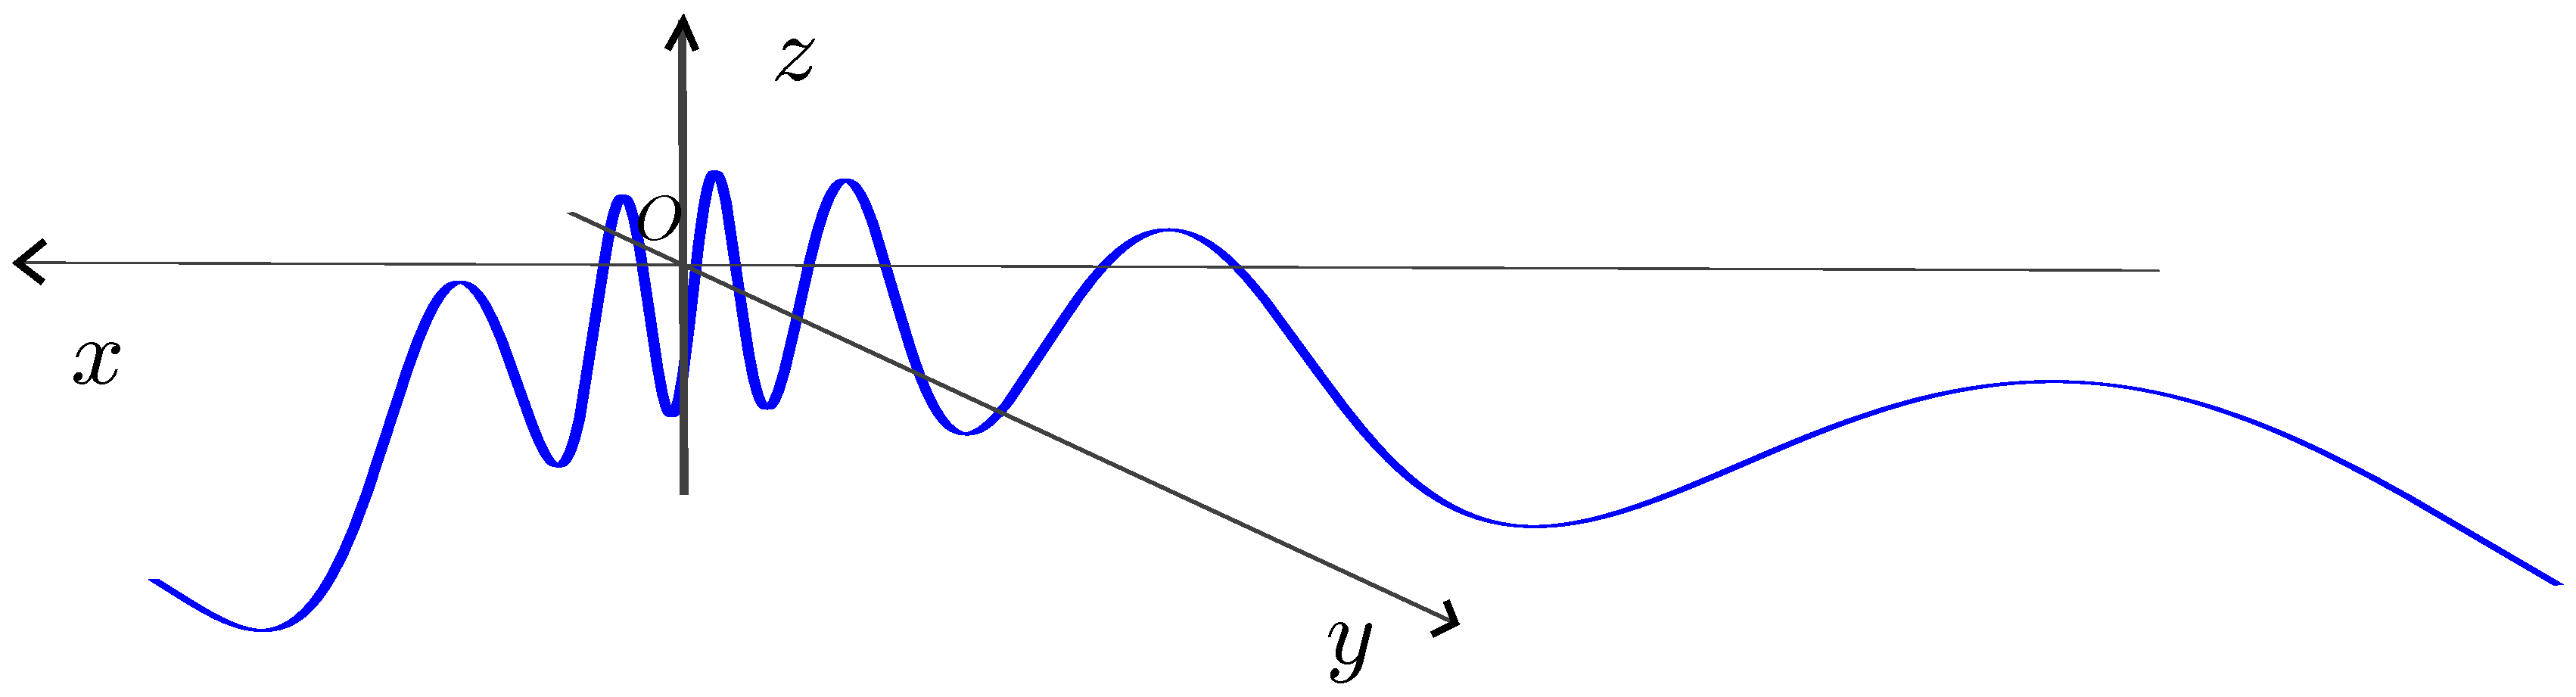
\includegraphics[width=0.8\textwidth]{prostorovekrivky-teorie3.eps}
	\caption{Křivka \textit{k} pro $t \in \langle-\pi, \pi\rangle$}
\end{figure}
\noindent Stejně jako u rovinných křivek mohou na prostorových křivkách být singulární body nebo uzlové body. Tečný vektor v singulárním bodě $K(t_0)$ buď neexistuje nebo je nulový, tj.:
$$k'(t_0)=(0,0,0).$$
\clearpage
\subsection*{Příklad 1}
Je dána křivka
$$k(t) = [\cos^3{t}, \sin^3{t}, \cos{2t}], t \in \langle0, 2\pi\rangle.$$
Napište souřadnice singulárních bodů. Dále popište tečnu křivky v bodě $T=k\left(\frac{\pi}{6}\right)$. \\[10pt]
\textbf{Řešení:} Vypočítáme tečné vektory
$$k'(t)=(-3 \cos^2{t} \cdot \sin{t}, 3 \sin^2{t} \cdot \cos{t}, -2\sin{2t}).$$
Má-li být nějaký bod singulární, musí být tečný vektor nulový. \\
Řešíme soustavu rovnic na intervalu $\langle0,2\pi\rangle$:
\begin{align*}
	-3\cos^2{t}\sin{t} & = 0, \\
	3\sin^2{t}\cos{t}  & = 0, \\
	-2\sin{2t}         & = 0. 
\end{align*}
Můžeme najít řešení všech tří rovnic na intervalu $\langle0,2\pi\rangle$ a pak udělat průnik řešení. Výhodnější je
najít všechna řešení jedné rovnice na intervalu $\langle0,2\pi\rangle$ a do zbývajících 2 rovnic tato řešení dosadit.
Vybereme ta řešení, která vyhovují pro všechny rovnice. \\
Vybereme si poslední rovnici
\begin{align*}
	\sin{2t} & = 0              \\
	2t       & = k\pi           \\
	t        & = k\frac{\pi}{2} 
\end{align*}
Na intervalu $\langle0,2\pi\rangle$ máme 5 řešení
$$t \in \left\{0, \frac{\pi}{2}, \pi, \frac{3\pi}{2}, 2\pi\right\}$$
Všech 5 řešení vyhovuje i zbývajícím rovnicím. Máme 4 singulární body
\begin{align*}
	S_1 & = k(0) = k(2\pi)=[1,0,1],                   \\
	S_2 & = k\left(\frac{\pi}{2}\right) = [0,1,-1],   \\
	S_3 & = k(\pi) = [-1,0,1],                        \\
	S_4 & = k\left(\frac{3\pi}{2}\right) = [0,-1,-1]. 
\end{align*}
Tečný vektor v bodě $T=k\left(\frac{\pi}{6}\right)=\left[\frac{3\sqrt{3}}{8}, \frac{1}{8}, \frac{1}{2}\right]$
je $k'\left(\frac{\pi}{6}\right)=\left(-\frac{9}{8},\frac{3\sqrt{3}}{8},-\sqrt{3}\right)$, ten můžeme nahradit vektorem $(3\sqrt{3}, -3, 8)$. \\
Tečna \textit{p} křivky \textit{k} v bodě \textit{T} je
$$p(s)=\left[\frac{3\sqrt{3}}{8}+3\sqrt{3}s, \frac{1}{8}-3s, \frac{1}{2}+8s\right], s \in \mathbb{R}.$$
\begin{figure}[H]
	\centering
	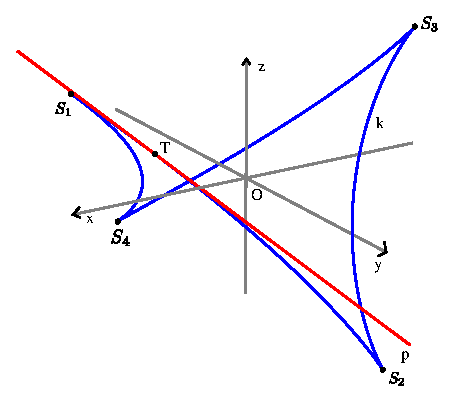
\includegraphics[width=0.8\textwidth]{prostorovakrivka1.eps}
	\caption{Prostorová křivka  pro $t \in \langle0, 2\pi\rangle$}
	\label{overflow}
\end{figure}
\clearpage
\subsection*{Příklad 2}
Je dána křivka
$$k(t) = \left[\frac{1}{2}\sin{2t}, \sin{t}, \cos{t}\right], t \in \langle0, 2\pi\rangle.$$
Napište souřadnice singulárních bodů. Dále popište tečnu křivky v bodě $T=k\left(0\right)$
a napište rovnici normálové roviny v bodě \textit{T}. \\
\textbf{Poznámka:} Normálová rovina v bodě \textit{T} je množina všech přímek (normál), které procházejí
bodem \textit{T} a jsou kolmé k tečně v bodě \textit{T}. \\[10pt]
\textbf{Řešení:} Vypočítáme tečné vektory
$$k'(t)=(\cos{2t}, \cos{t}, -\sin{t}).$$
Pro singulární body řešíme soustavu rovnic na intervalu $\langle0,2\pi\rangle$:
\begin{align*}
	\cos{2t} & = 0, \\
	\cos{t}  & = 0, \\
	-\sin{t} & = 0. 
\end{align*}
Druhá a třetí rovnice nejsou splněny zároveň pro žádné \textit{t}. Křivka nemá singulární body. \\
Tečný vektor v bodě $T=k(0)=[0,0,1]$ je vektor $k'(0)=(1,1,0)$.
Tečna \textit{p} křivky \textit{k}\\ v bodě \textit{T} je
$$p(s)=[s,s,1], s \in \mathbb{R}.$$
Tečný vektor $(1,1,0)$ je vektor kolmý k hledané normálové rovině $\alpha$. \\
Rovina $\alpha$ má rovnici $x+y+d=0$, číslo \textit{d} určíme dosazením bodu \textit{T}, $d=0$, 
$$\alpha: x+y=0.$$
\begin{figure}[ht!]
	\centering
	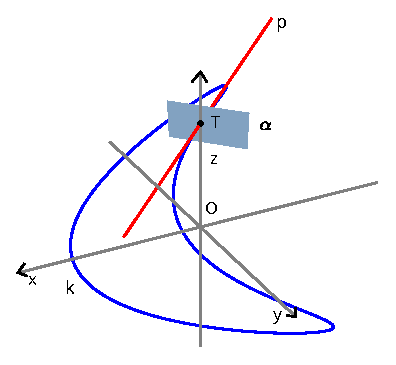
\includegraphics[width=0.8\textwidth]{prostorovakrivka2.eps}
	\caption{Prostorová křivka  pro $t \in \langle0, 2\pi\rangle$}
	\label{overflow}
\end{figure}
\clearpage
\subsection*{Příklad 3}
Je dána křivka
$$k(t) = [\cos{3t}, \sin{2t}, \cos{4t}], t \in \langle0, 2\pi\rangle.$$
Popište tečnu křivky v bodě $T=k\left(0\right)$
a napište rovnici normálové roviny v bodě \textit{T}. \\[10pt]
\begin{figure}
	\centering
	\begin{subfigure}[b]{0.3\textwidth}
		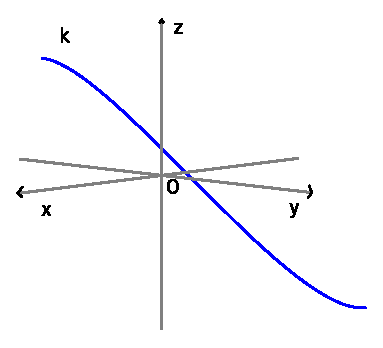
\includegraphics[width=\textwidth]{prostorovakrivka3-pi4.eps}
		\caption{$t \in \left\langle0, \frac{\pi}{4}\right\rangle$}
	\end{subfigure}%
	\begin{subfigure}[b]{0.3\textwidth}
		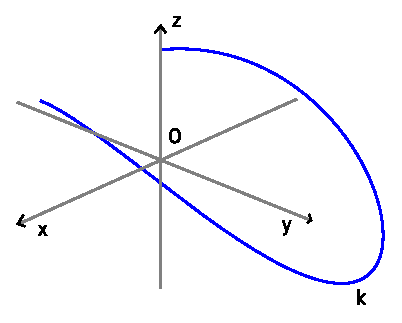
\includegraphics[width=\textwidth]{prostorovakrivka3-pi2.eps}
		\caption{$t \in \left\langle0, \frac{\pi}{2}\right\rangle$}
	\end{subfigure}
	\begin{subfigure}[b]{0.3\textwidth}
		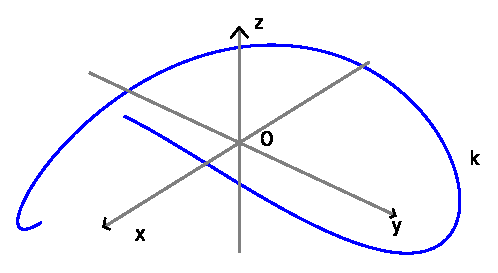
\includegraphics[width=\textwidth]{prostorovakrivka3-3pi4.eps}
		\caption{$t \in \left\langle0, \frac{3\pi}{4}\right\rangle$}
	\end{subfigure}
	\begin{subfigure}[b]{0.3\textwidth}
		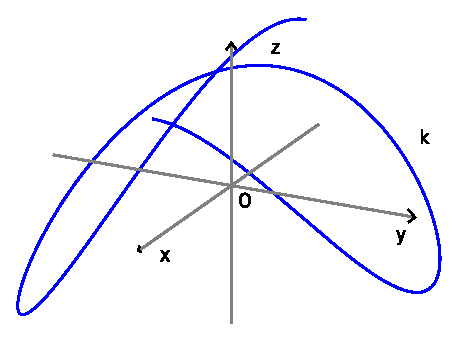
\includegraphics[width=\textwidth]{prostorovakrivka3-pi.eps}
		\caption{$t \in \langle0, \pi\rangle$}
	\end{subfigure}%
	\begin{subfigure}[b]{0.3\textwidth}
		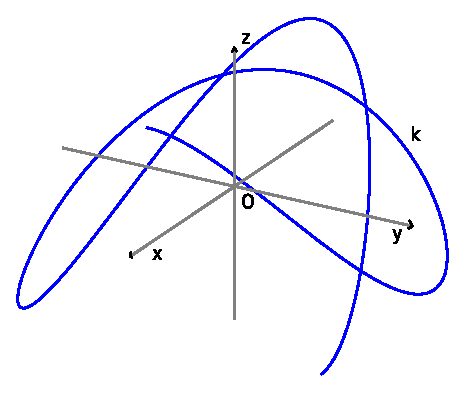
\includegraphics[width=\textwidth]{prostorovakrivka3-5pi4.eps}
		\caption{$t \in \left\langle0, \frac{5\pi}{4}\right\rangle$}
	\end{subfigure}
	\begin{subfigure}[b]{0.3\textwidth}
		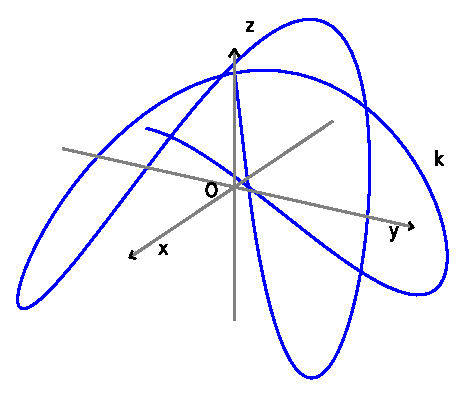
\includegraphics[width=\textwidth]{prostorovakrivka3-3pi2.eps}
		\caption{$t \in \left\langle0, \frac{3\pi}{2}\right\rangle$}
	\end{subfigure}
	\begin{subfigure}[b]{0.3\textwidth}
		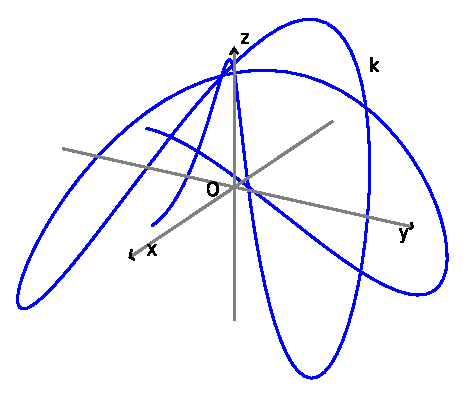
\includegraphics[width=\textwidth]{prostorovakrivka3-7pi4.eps}
		\caption{$t \in \left\langle0, \frac{7\pi}{4}\right\rangle$}
	\end{subfigure}
	\begin{subfigure}[b]{0.3\textwidth}
		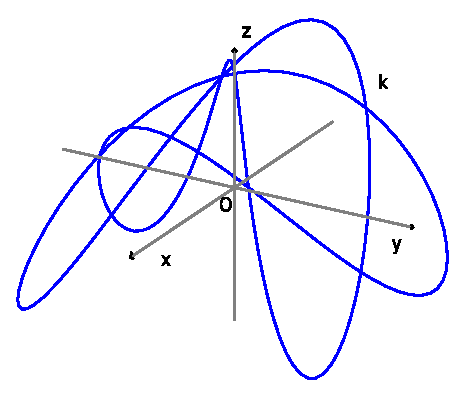
\includegraphics[width=\textwidth]{prostorovakrivka3-2pi.eps}
		\caption{$t \in \langle0, 2\pi\rangle$}
	\end{subfigure}
	\caption{Prostorová křivka \textit{k} pro různé intervaly parametru \textit{t}}
\end{figure}
\textbf{Řešení:} Vypočítáme tečné vektory
$$k'(t)=(-3\sin{3t}, 2\cos{2t}, -4\sin{4t}).$$
Tečný vektor v bodě $T=k(0)=[1,0,1]$ je vektor $k'(0)=(0,2,0)$ (ten můžeme v popisu tečny nahradit vektorem $(0,1,0)$).
Tečna \textit{p} křivky \textit{k} v bodě \textit{T} je
$$p(s)=[1,s,1], s \in \mathbb{R}.$$
Tečný vektor $(0,1,0)$ je vektor kolmý k hledané normálové rovině $\alpha$. \\
Rovina $\alpha$ má rovnici $y+d=0$, číslo \textit{d} určíme dosazením bodu \textit{T}, $d=0$, 
$$\alpha: y=0,$$
Je to rovina $(x, z)$.
\begin{figure}[ht!]
	\centering
	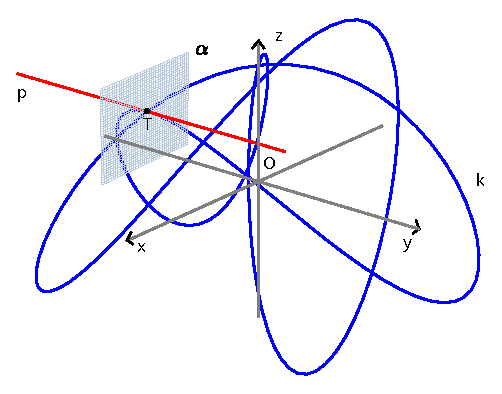
\includegraphics[width=0.8\textwidth]{prostorovakrivka3.eps}
	\caption{Tečna a normálová rovina křivky \textit{k} ($t \in \langle0, 2\pi\rangle$)}
	\label{overflow}
\end{figure}
\clearpage
\subsection*{Příklad 4}
Je dána křivka
$$k(t) = [\sin{2t}, 1 - \cos{2t}, 2\cos{t}], t \in \langle0, 2\pi\rangle.$$
Zjistěte, zda má křivka uzlový bod. Pokud ano, popište všechny tečny v tomto bodě.
Pokud všechny tečny v uzlovém bodě leží v jedné rovině, napište obecnou rovnici této roviny. \\[10pt]
\textbf{Řešení:} Z předpisu křivky $k(t) = [\sin{2t}, 1 - \cos{2t}, 2\cos{t}]$ můžeme získat 3 rovinné křivky. \\
Křivka \textit{l} v rovině $(x, y)$
$$l(t) = [\sin{2t}, 1 - \cos{2t}, 0], t \in \langle0, 2\pi\rangle.$$
je pravoúhlý průmět křivky \textit{k} do roviny $(x,y)$ (tzv. půdorys křivky \textit{k}). \\
Křivka \textit{m} v rovině $(y, z)$
$$m(t) = [0, 1 - \cos{2t}, 2\cos{t}], t \in \langle0, 2\pi\rangle$$
je pravoúhlý průmět křivky \textit{k} do roviny $(y,z)$ (tzv. bokorys křivky \textit{k}). \\
Křivka \textit{n} v rovině $(x, z)$
$$n(t) = [\sin{2t}, 0, 2\cos{t}], t \in \langle0, 2\pi\rangle$$
je pravoúhlý průmět křivky \textit{k} do roviny $(y,z)$ (tzv. nárys křivky \textit{k}). \\
Zajímavá je pro nás křivka \textit{l}, ve které snadno rozpoznáme kružnici o středu $S=[0,1,0]$
a poloměru $r=1$.Tato kružnice je při $t \in \langle0, 2\pi\rangle$ oběhnuta dvakrát. \\
\begin{figure}[H]
	\centering
	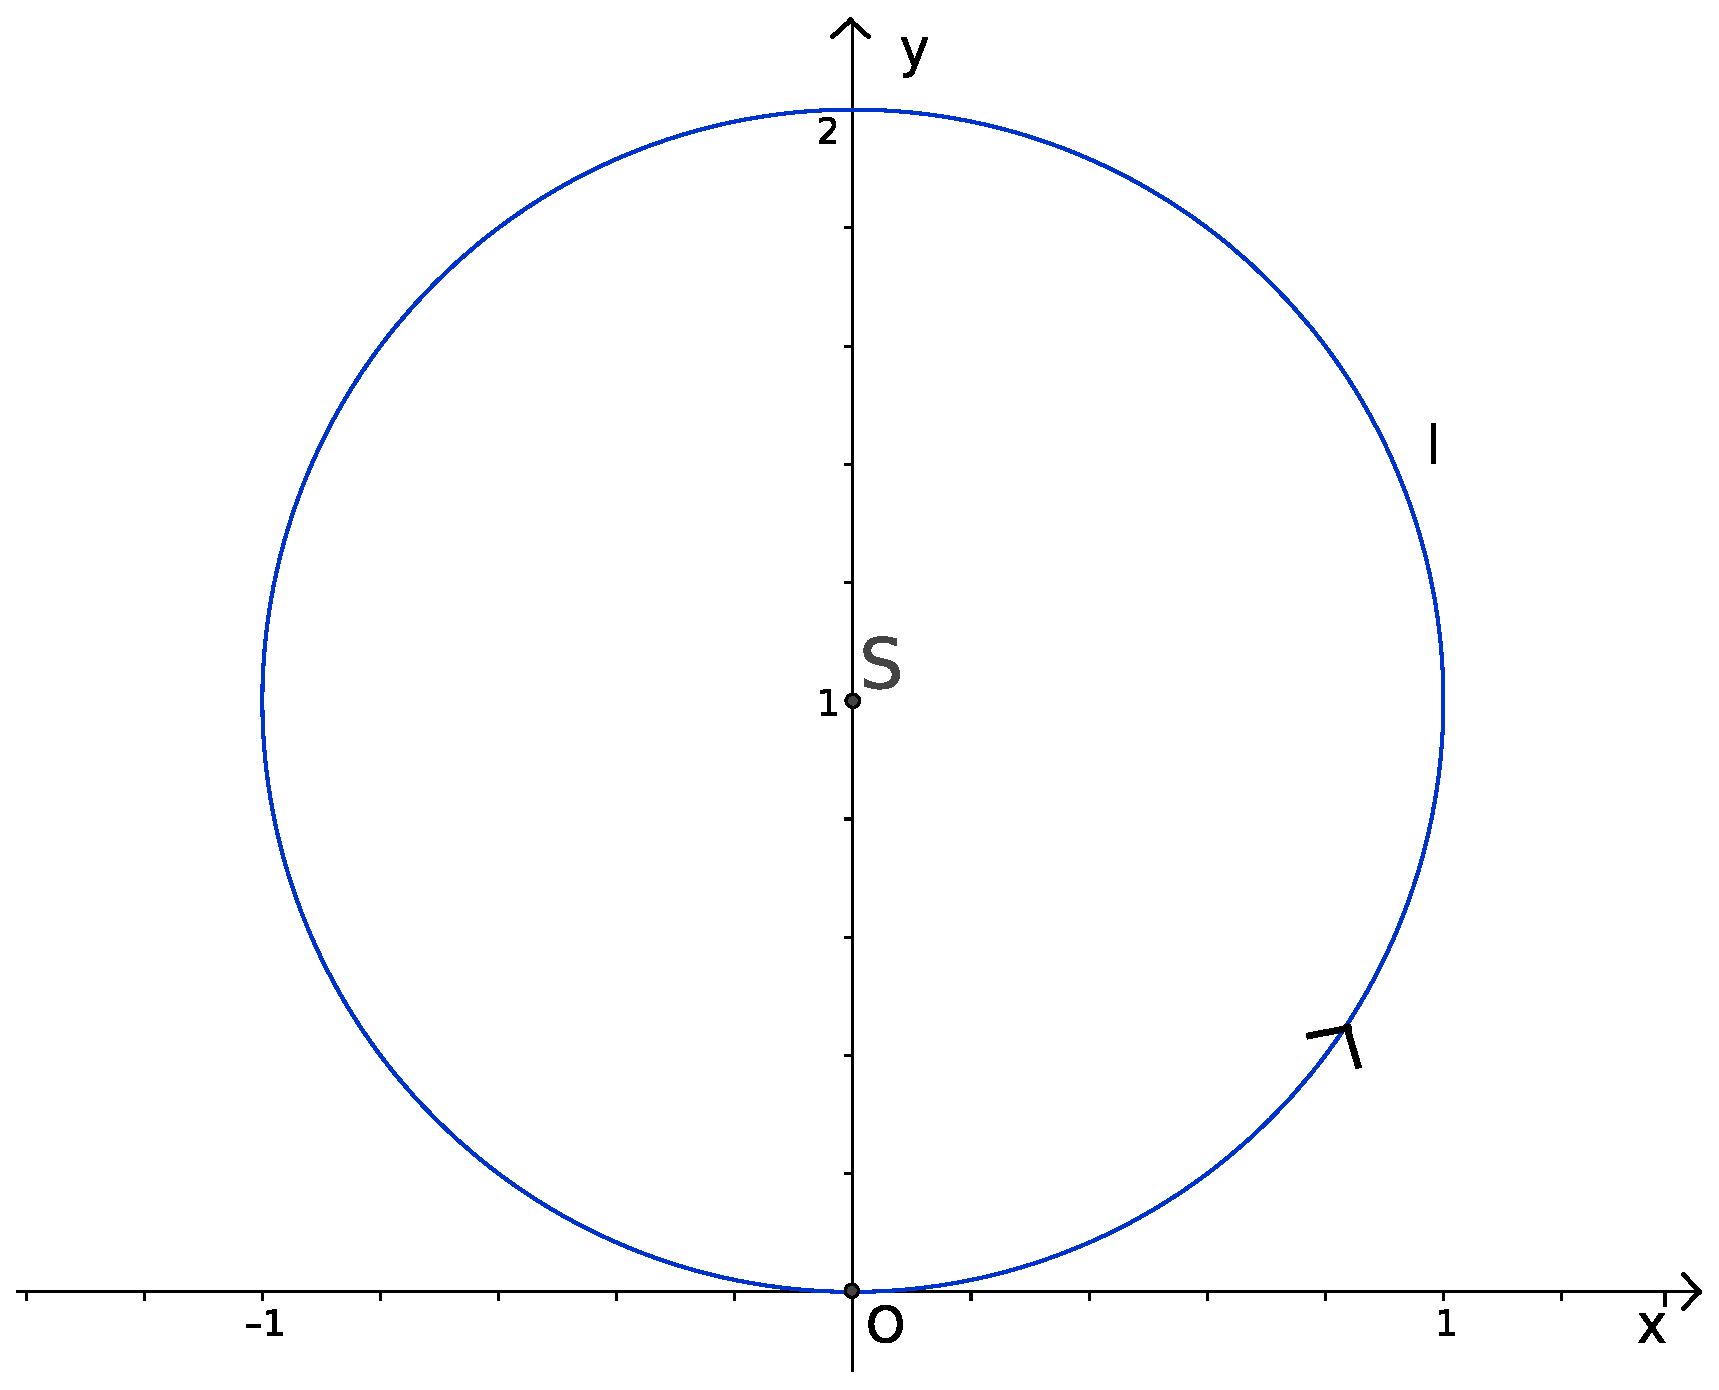
\includegraphics[width=0.4\textwidth]{prostorovakrivka3-l.eps}
	\caption{Půdorys křivky \textit{k} pro $t \in \langle0, 2\pi\rangle$}
	\label{overflow}
\end{figure}
Křivka \textit{k} leží na rotační válcové ploše, kružnice \textit{l} je její řídící kružnice, 
osa válcové plochy je přímka \textit{o} rovnoběžná s osou \textit{z}. \\
Třetí \textit{z}-ové souřadnice křivky \textit{k} jsou kladné pro $t \in \left\langle0, \frac{\pi}{2}\right)$,
záporné pro $t \in \left(\frac{\pi}{2}, \frac{3\pi}{2}\right)$ a kladné pro $t \in \left(\frac{3\pi}{2}, 2\pi\right\rangle)$.\\
Pro intervaly $\left\langle0, \frac{\pi}{2}\right)$ a $\left\langle\pi, \frac{3\pi}{2}\right)$ (pravá polovina kružnice \textit{l})
má křivka \textit{k} různě \textit{z}-ové souřadnice. Stejně je tomu tak pro intervaly $\left(\frac{\pi}{2}, \pi\right\rangle$ a
$\left(\frac{3\pi}{2}, 2\pi\right\rangle$ (levá polovina kružnice \textit{l}). \\
Stejné souřadnice při různých hodnotách parametru \textit{t} jsou pouze
\begin{align*}
	k(0)                        & = k(2\pi) = [0,0,2] = T,                      \\
	k\left(\frac{\pi}{2}\right) & = k\left(\frac{3\pi}{2}\right) = [0,2,0] = U. 
\end{align*}
Vypočteme tečné vektory
$$k'(t) = (2\cos{2t}, 2\sin{2t}, -2\sin{t}).$$
a dosadíme
\begin{align*}
	k'(0)                         & = k'(2\pi) = (2,0,0),     \\
	k'\left(\frac{\pi}{2}\right)  & = (-2,0,-2) \sim (1,0,1), \\
	k'\left(\frac{3\pi}{2}\right) & = (-2,0,2) \sim (1,0,-1). 
\end{align*}
V bodě \textit{T} je jen jedna tečna rovnoběžná s osou \textit{x}. Křivka začíná a končí v jednom bodě \textit{T},
křivka je uzavřená. V uzlovém bodě \textit{U} má křivka dvě různé tečny:
\begin{align*}
	p(s) & = [s,2,s], s \in \mathbb{R},  \\
	q(u) & = [u,2,-u], u \in \mathbb{R}. 
\end{align*}
Tyto tečny určují rovinu:
$$\alpha: y-2=0.$$
Podívejme se ještě na křivky \textit{m} a \textit{n}, tedy na bokorys a nárys křivky \textit{k}. \\
Křivku $m(t) = [0, 1 - \cos{2t}, 2\cos{t}], t \in \langle0, 2\pi\rangle$ upravme
$$m(t) = [0, 1 - \cos^2{t}+\sin^2{t}, 2\cos{t}] = [0, 2-2\cos^2{t}, 2\cos{t}].$$
a provedeme substituci $v=\cos{t}$. Dostaneme jinou parametrizaci křivky \textit{m}:
$$m(v) = [0, 2-2v^2, 2v], v \in \langle-1, 1\rangle.$$
Odsud již vidíme, že bokorysem křivky \textit{k} je část paraboly. \\
\begin{figure}[H]
	\centering
	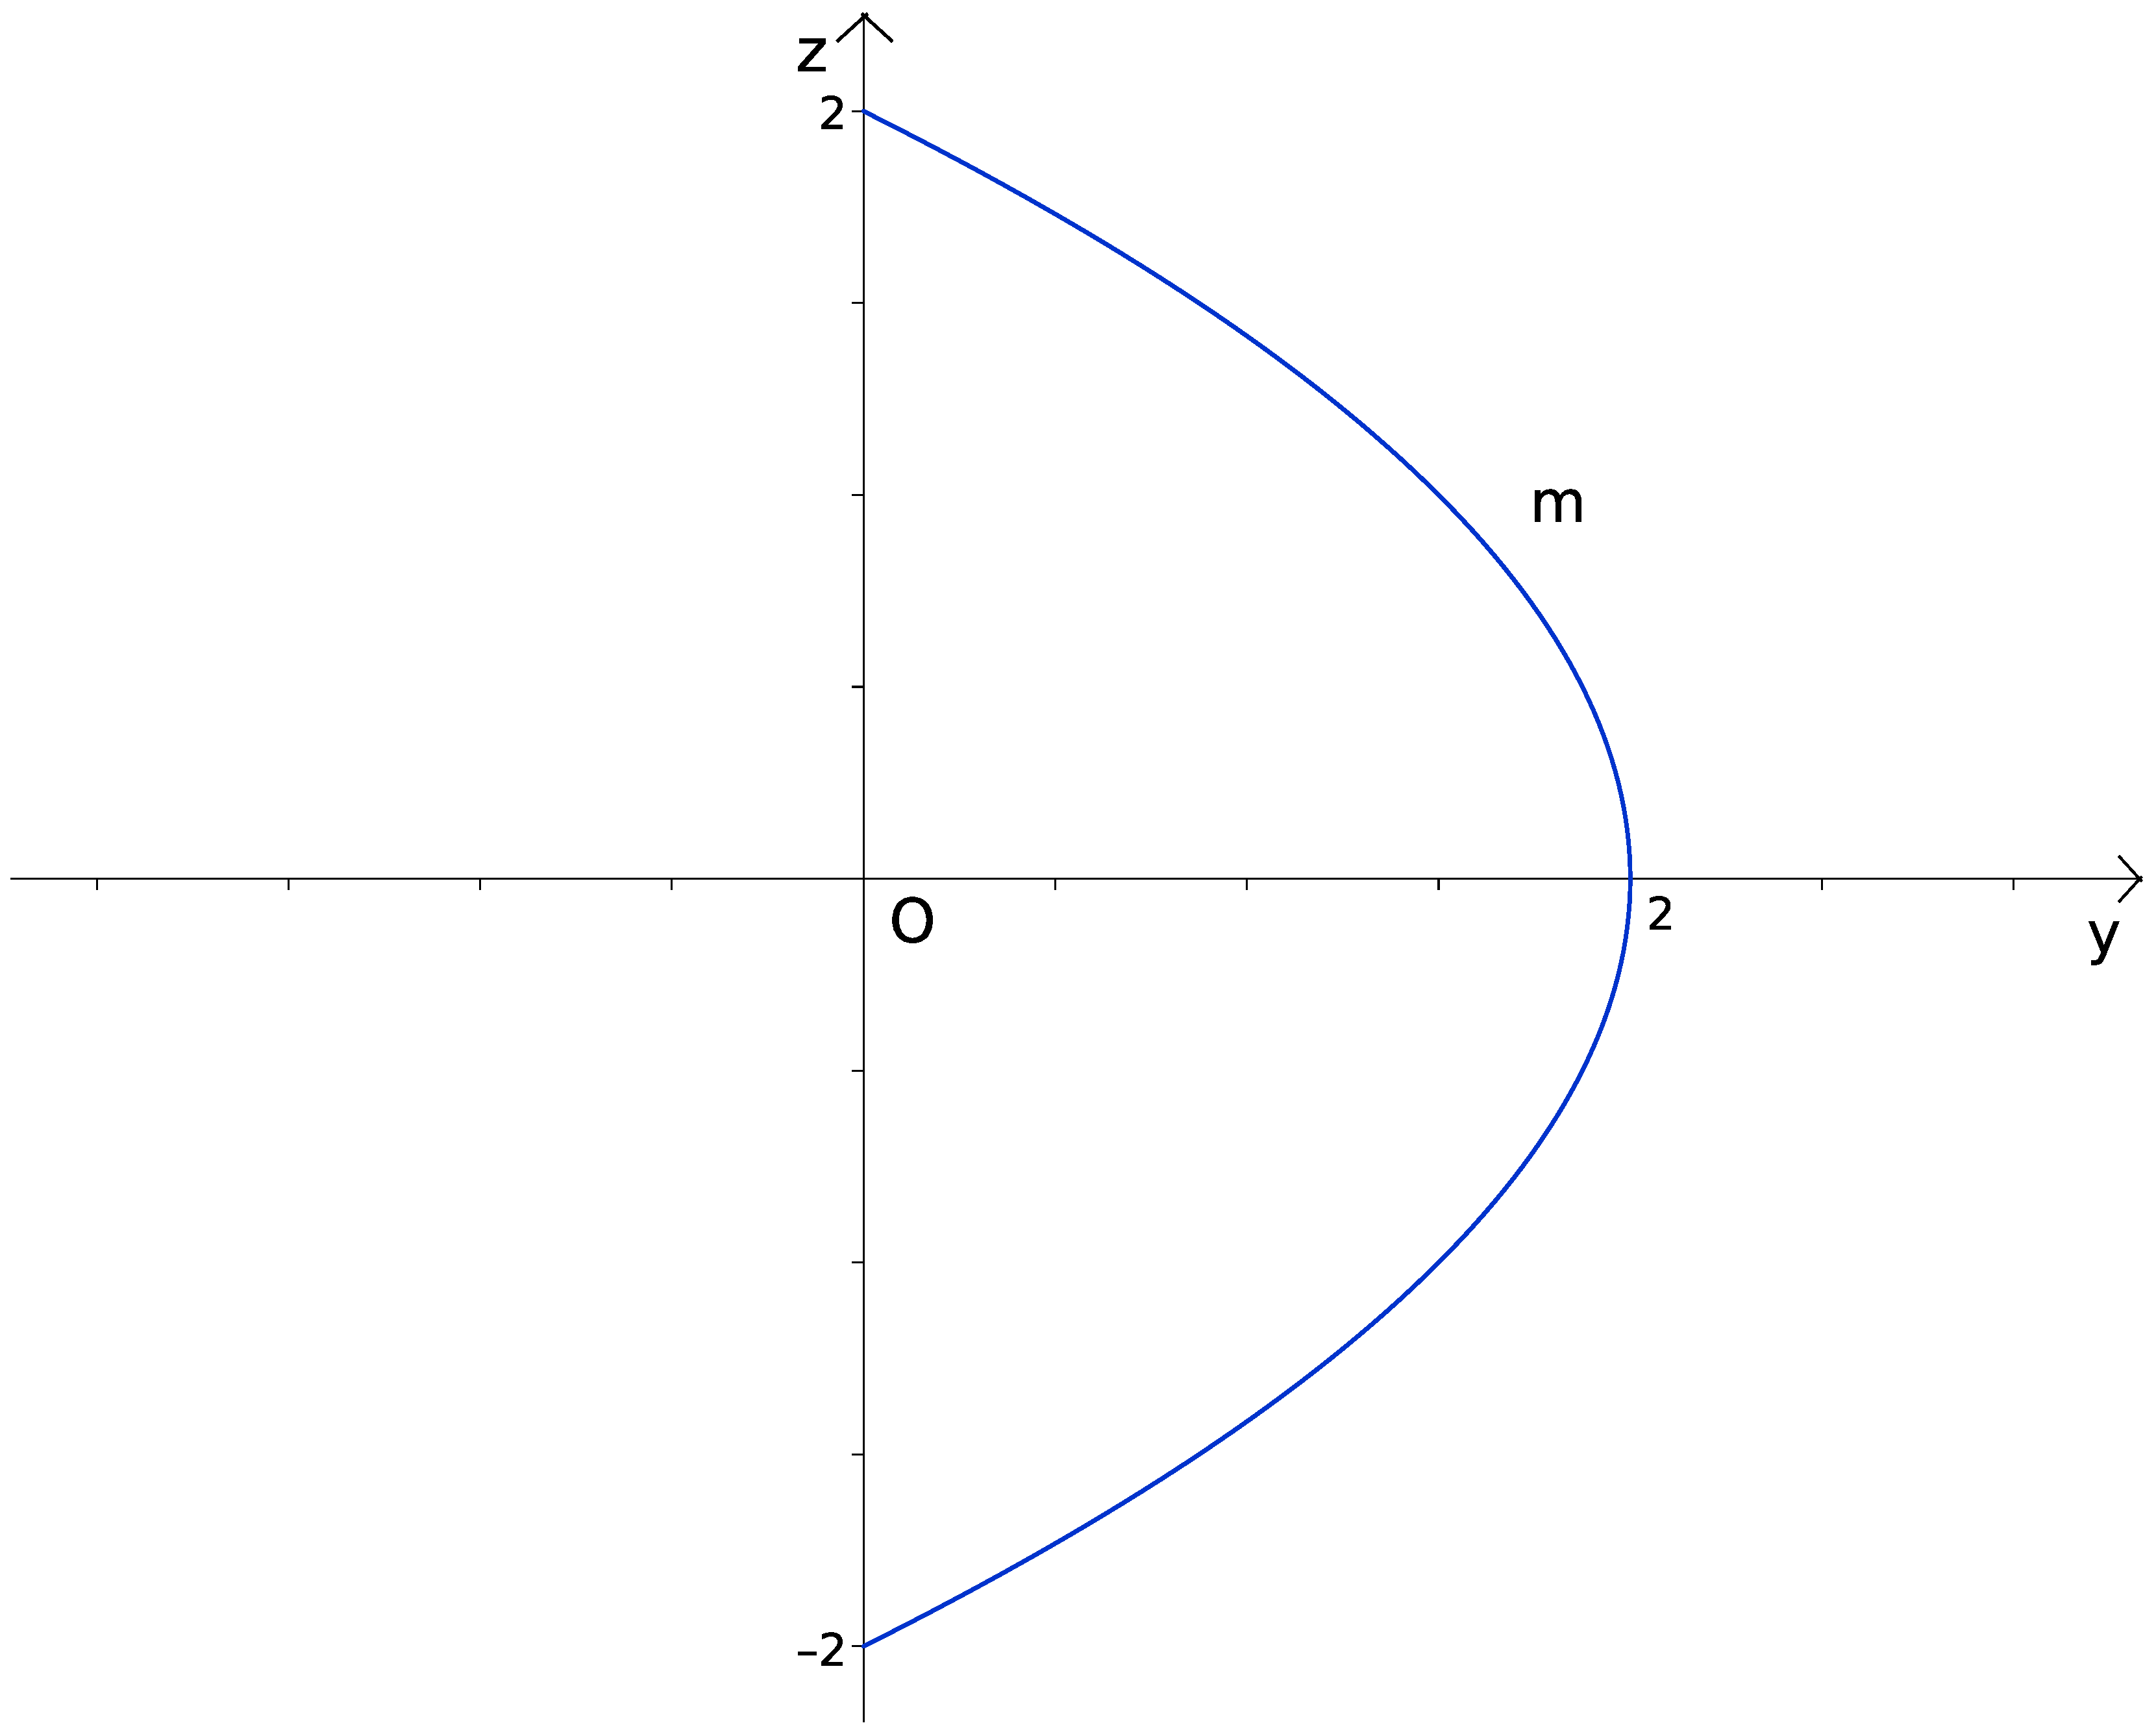
\includegraphics[width=0.4\textwidth]{prostorovakrivka3-m.eps}
	\caption{Bokorys křivky \textit{k} pro $t \in \langle0, 2\pi\rangle$}
	\label{overflow}
\end{figure}
Křivku $n(t) = [\sin{2t}, 0, 2\cos{t}], t \in \langle0, 2\pi\rangle$ nakreslíme s využitím grafického programu.
Z tohoto obrázku je již zřejmé, že křivka má uzlový bod. \\
\begin{figure}[H]
	\centering
	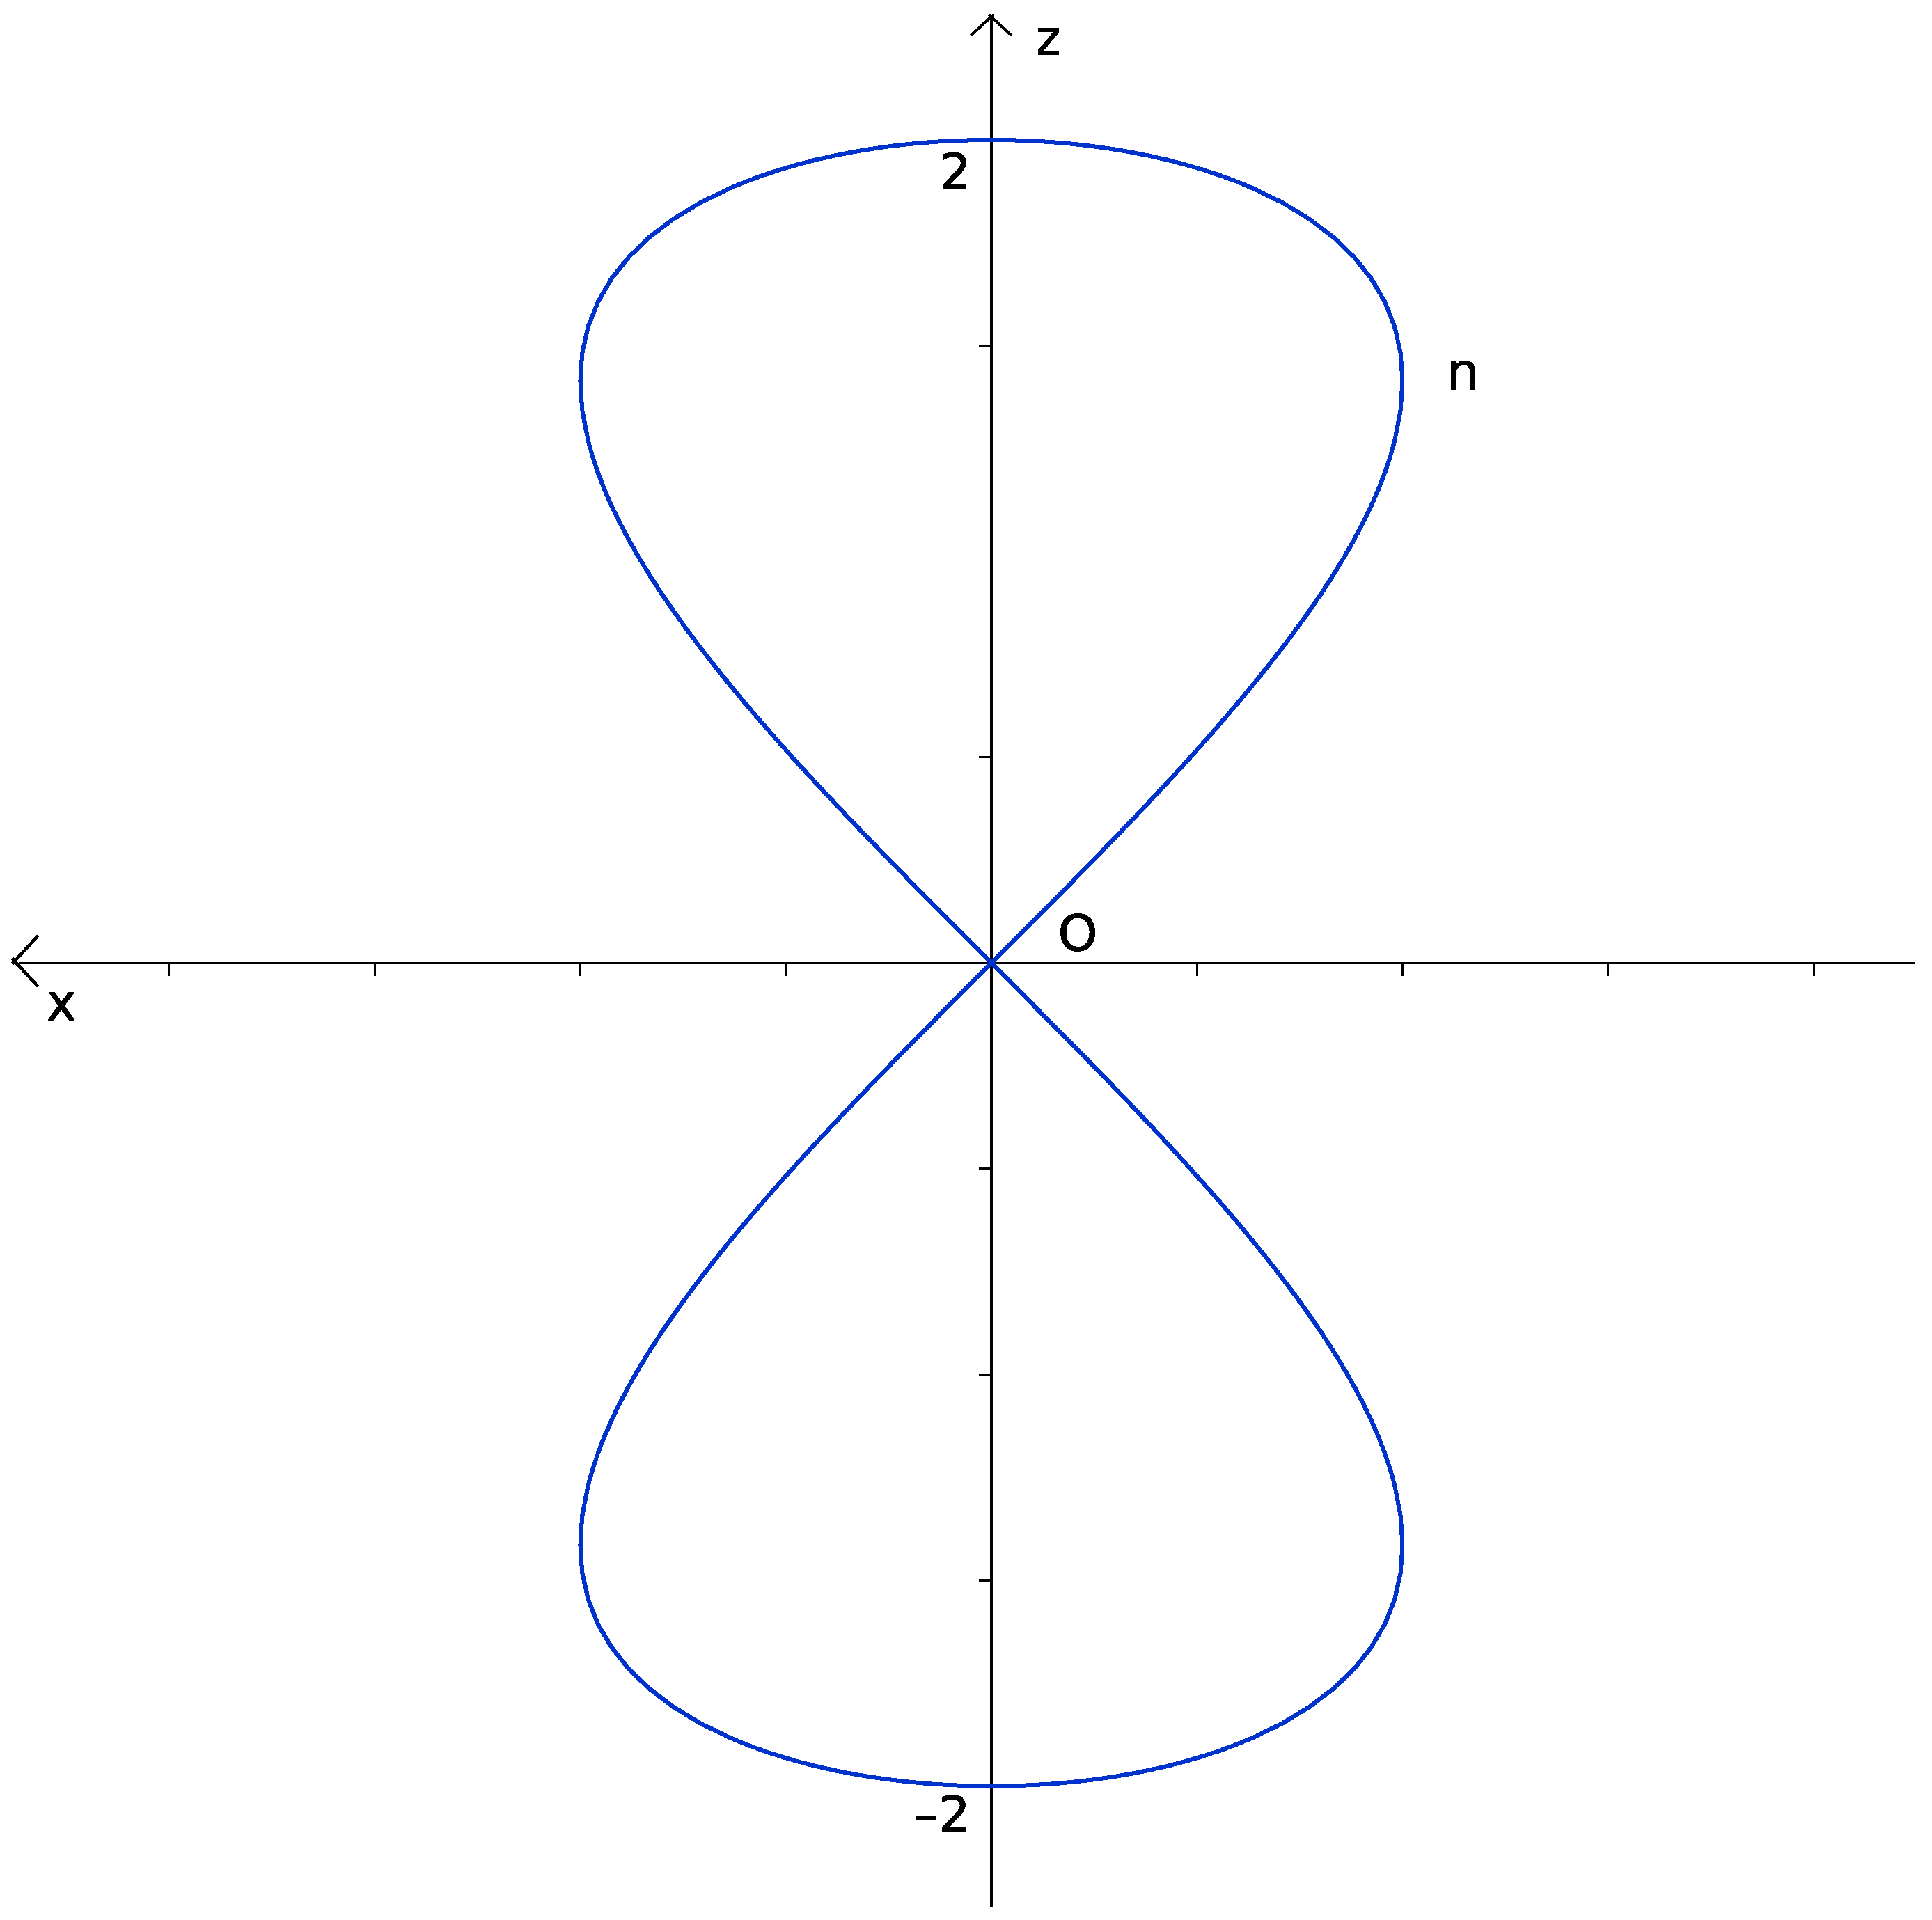
\includegraphics[width=0.4\textwidth]{prostorovakrivka3-n.eps}
	\caption{Nárys křivky \textit{k} pro $t \in \langle0, 2\pi\rangle$}
	\label{overflow}
\end{figure}
Křivka \textit{k} se nazývá \textit{Vivianiho křivka} (nebo také \textit{Vivianiho okénko}) a je průnikem
válcové plochy $x^2+(y-1)^2=1$ a kulové plochy $x^2+y^2+z^2=4$. Viz práce studenta Michala Šestáka: Parametrické
vyjádření rotačních a šroubových ploch.
\begin{figure}[H]
	\centering
	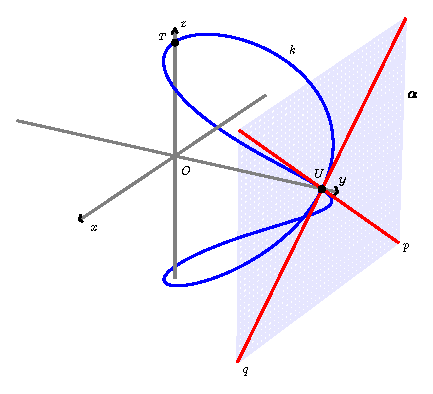
\includegraphics[width=\textwidth]{prostorovakrivka4.eps}
	\caption{Křivka \textit{k} pro $t \in \langle0, 2\pi\rangle$}
	\label{overflow}
\end{figure} 
